\documentclass[border=10pt]{standalone}

\usepackage{tikz}
\usepackage{tikzsymbols}
\usetikzlibrary{calc,patterns,shapes.geometric}

\def\centerarc[#1](#2)(#3:#4:#5){\draw[#1] ($(#2)+({#5*cos(#3)},{#5*sin(#3)})$) arc (#3:#4:#5);}

\begin{document}
	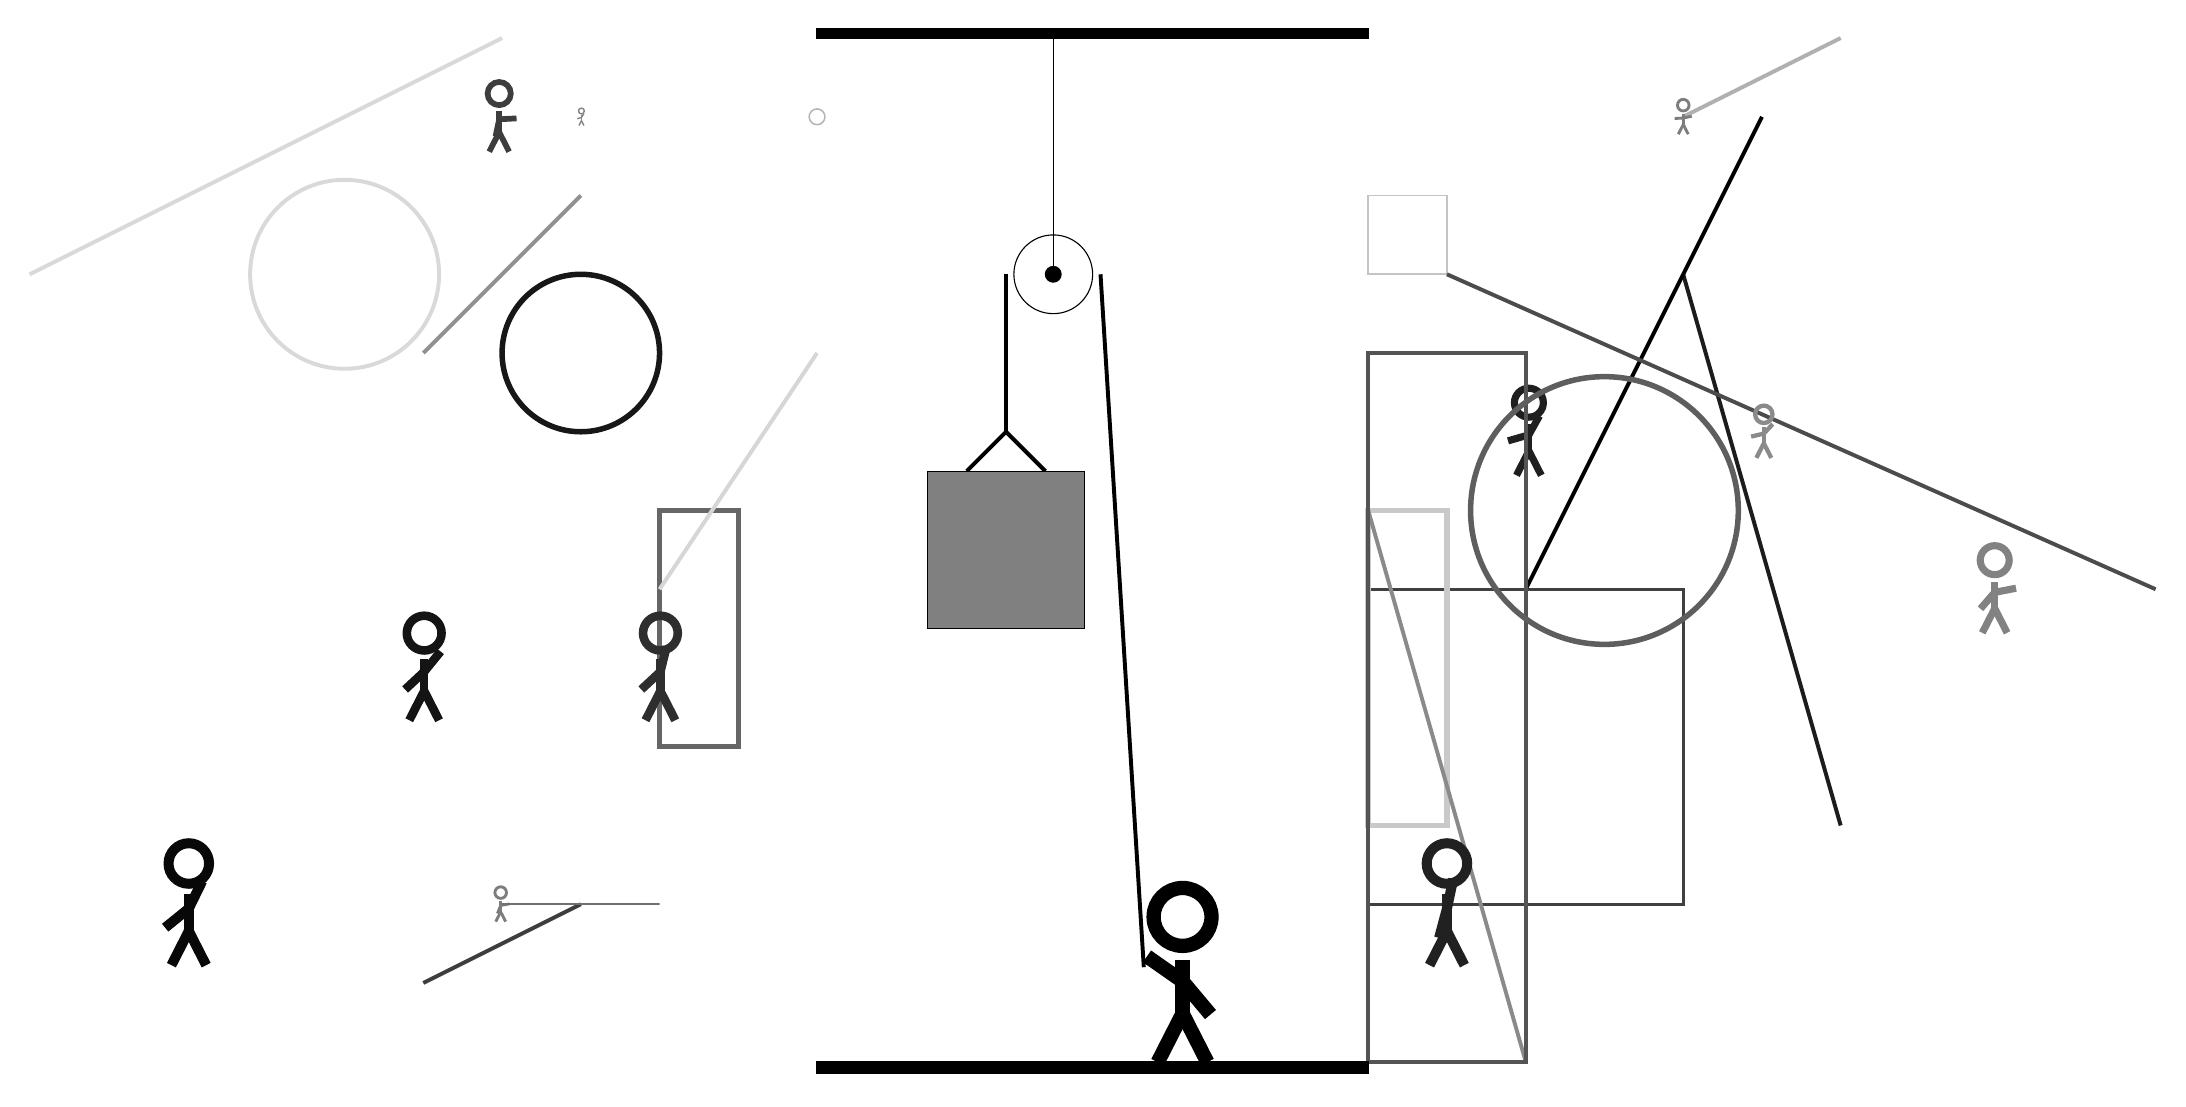
\begin{tikzpicture}
		%%%%% START %%%%%
		
		\draw[fill=black] (-2, 10) rectangle (5, 10.125);
		
		\draw (1, 7) circle (0.5);
		\draw[fill=black] (1, 7) circle (0.1);
		\draw (1, 10) -- (1, 7);
		
		\draw[line width=0.5mm] (-0.1, 4.5) -- (0.4, 5.0) -- (0.9, 4.5);
		\draw[fill=black!50] (-0.6, 4.5) rectangle (1.4, 2.5);
		
		\draw[line width=0.7mm, color=black!60] (-3, 1) rectangle (-4, 4);
		
		\draw[line width=0.5mm, color=black!16](-2, 6) -- (-4, 3);
		\draw[line width=0.5mm, color=black!89](9, 7) -- (11, 0);
		\draw[line width=0.4mm, color=black!75] (5, 3) rectangle (9, -1);
		\draw[line width=0.7mm, color=black!21] (6, 0) rectangle (5, 4);
		
		\node[line width=0.3mm, color=black!51] at (-6, -1) {\Strichmaxerl[2][68][10]};
		
		\draw[line width=0.2mm, color=black!23] (6, 8) rectangle (5, 7);
		\node[line width=0.2mm, color=black!88] at (7, 5) {\Strichmaxerl[5][16][61]};
		\node[line width=0.7mm, color=black!82] at (-4, 2) {\Strichmaxerl[6][43][76]};
		\node[line width=0.3mm, color=black!97] at (-10, -1) {\Strichmaxerl[7][39][64]};
		\draw[line width=0.5mm, color=black!31](9, 9) -- (11, 10);
		\node[line width=0.6mm, color=black!49] at (13, 3) {\Strichmaxerl[5][49][11]};
		\node[line width=0.7mm, color=black!76] at (-6, 9) {\Strichmaxerl[4][78][3]};
		
		\draw[line width=0.5mm, color=black!100](10, 9) -- (7, 3);
		\draw[line width=0.5mm, color=black!46](7, -3) -- (5, 4);
		\node[line width=0.6mm, color=black!92] at (-7, 2) {\Strichmaxerl[6][43][51]};
		
		\node[line width=0.6mm, color=black!87] at (6, -1) {\Strichmaxerl[7][75][78]};
		\draw [line width=0.5mm, color=black!15](-8, 7) circle (1.2);
		\draw[line width=0.5mm, color=black!70](6, 7) -- (15, 3);
		
		\draw[line width=0.5mm, color=black!76](-5, -1) -- (-7, -2);
		\draw[line width=0.5mm, color=black!15](-6, 10) -- (-12, 7);
		\node[line width=0.5mm, color=black!46] at (10, 5) {\Strichmaxerl[3][13][47]};
		\node[line width=0.7mm, color=black!51] at (9, 9) {\Strichmaxerl[2][3][12]};
		\draw[line width=0.5mm, color=black!67] (7, -3) rectangle (5, 6);
		\draw [line width=0.7mm, color=black!91](-5, 6) circle (1.0);
		
		\draw [line width=0.2mm, color=black!29](-2, 9) circle (0.1);
		\draw [line width=0.7mm, color=black!63](8, 4) circle (1.7);
		\draw[line width=0.3mm, color=black!56] (-4, -1) rectangle (-6, -1);
		\node[line width=0.7mm, color=black!48] at (-5, 9) {\Strichmaxerl[1][18][57]};
		
		\draw[line width=0.5mm, color=black!43](-7, 6) -- (-5, 8);
		
		\draw[line width=0.5mm] (0.4, 7) -- (0.4, 5.0);
		\centerarc[line width=0.5mm](1, 7)(0:180:0.6);
		\draw[line width=0.5mm](1.6, 7) -- (2.15, -1.8);
		
		\node at (2.6, -1.9) {\Strichmaxerl[10][-35][-50]};
		
		\draw[fill=black] (-2, -3) rectangle (5, -3.15);
		
		%%%%% END %%%%%
	\end{tikzpicture}
\end{document}